\documentclass[a4paper,10pt,twocolumn]{article}
\usepackage[margin=-1.34, left=2.1cm, right=2.5cm, top=2.1cm, bottom=2.5cm]{geometry}
\usepackage{caption}
\usepackage{graphicx}
\graphicspath{ {./images/} }
\newcommand{\RomanNumeralCaps}[1]
    {\MakeUppercase{\romannumeral #1}}
\begin{document} 
\setcounter{page}{288}
\vspace{-3 mm}
\hangindent=0.4cm radiologists and clinicians in the detection and characterization of breast lesions during ultrasound examinations.
  
\begin{figure}[h]
     \centering
     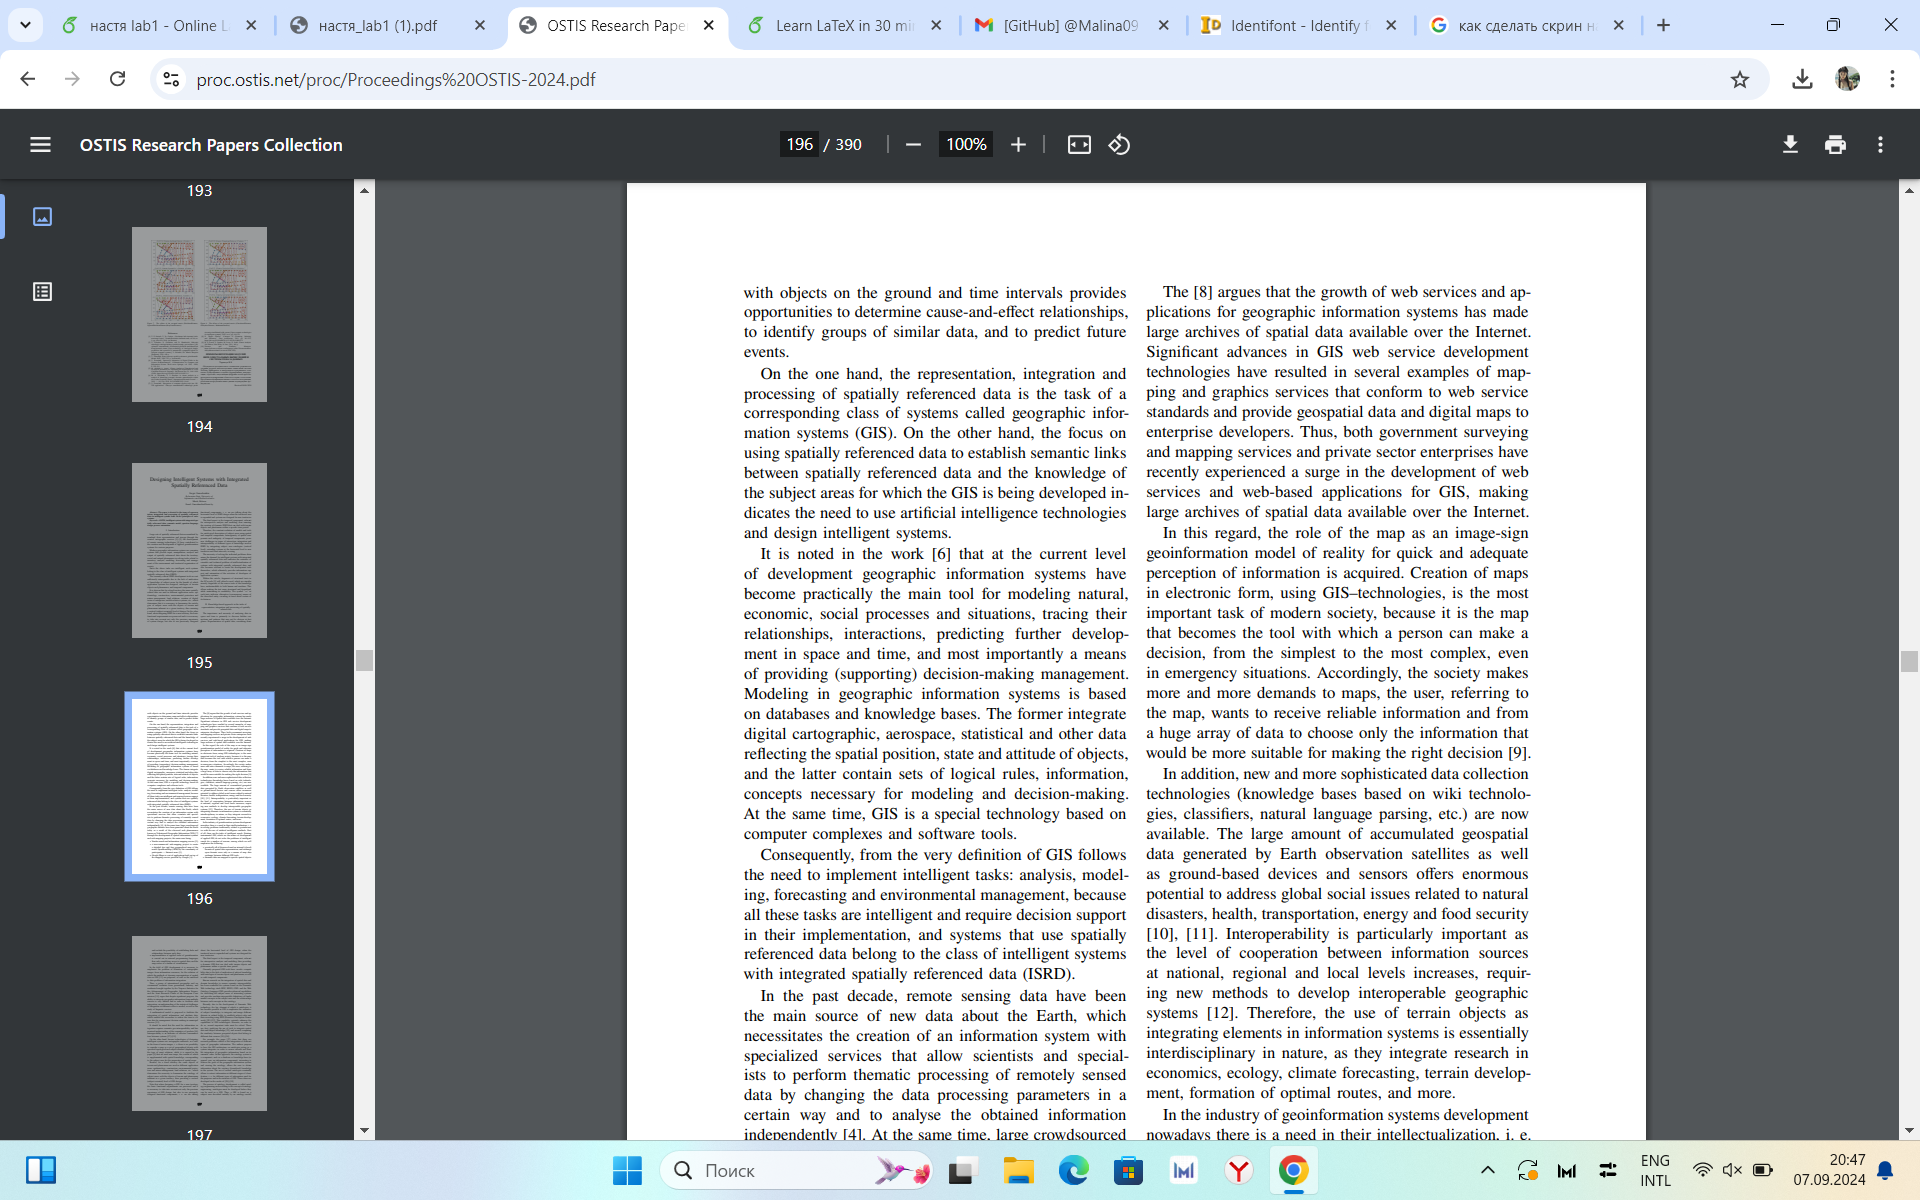
\includegraphics[width=1.0\columnwidth]{Снимок экрана (1).png}
      \caption{\scriptsize{An example of Samsung S-Detect-system interface [8]}}
      \label{fig:figure}
\end{figure} 

This system has a lot of pros: it provides real-time feedback to the clinician during the examination, enabling
immediate assessment and decision-making regarding
lesion characterization and management. More than that,
the software provides standardized reporting templates
that facilitate structured documentation of lesion characteristics, including malignancy probability scores and recommended management options. This promotes consistency and completeness in reporting. S-Detect seamlessly
integrates with the RS80A ultrasound system’s workflow,
allowing for efficient and streamlined use within clinical
practice. It is user-friendly and does not significantly
disrupt the examination process.

But S-Detect is primarily designed for breast lesion
characterization and may not be suitable for other types
of lesions or organs. Its utility is limited to breast
ultrasound examinations and may not address the full
spectrum of diagnostic challenges encountered in clinical practice. While S-Detect is user-friendly, clinicians
may require some time to familiarize themselves with
the software’s features and functionality. Training and
ongoing education may be necessary to optimize its
use and interpretation. Moreover, The implementation
of S-Detect may incur additional costs associated with
software licensing, training, and maintenance. Clinics
and healthcare facilities must consider the financial implications before adopting the technology.

There are another people who have been automating
ultrasound diagnostics of the thyroid gland using artificial intelligence. For example in 2021 scientists from
Romania published their article "Intelligent Diagnosis of
Thyroid Ultrasound Imaging Using an Ensemble of Deep
Learning Methods".

They developed a CNN-VGG ensemble fused from two
models: a pre-trained fined tuned model VGG-19 and an
efficient lightweight CNN model. The proposed ensemble
method proved to be an excellent and stable classifier
with a good performance in terms of overall sensitivity
(95.75\%), specificity (98.43\%), accuracy (97.35\%), AUC(0.96), positive predictive value (95.41\%) and negative
predictive value (98.05\%). [9]

Also there are scientists from China who published an
"Artificial intelligence in thyroid ultrasound" article in
2023. Their research is more focused on the prevention
and early detection of the thyroid cancer. They also used
deep learning algorithms to achieve this goal. They tests
different types of DL-based neural networks. [7]

The research of the above-mentioned scientists has
been very successful. Their authors placed great emphasis on training the neural network to make diagnoses and
look for pathology in ultrasound diagnostic images.

In the current work, a simpler and more global
approach is considered: the neural network does not
diagnose, but only assists the doctor. Their joint work
makes it possible to minimize the errors of both the
doctor and the software. The approach is described using
the example of thyroid gland examination, but it can also
be used in ultrasound diagnostics of other organs.

Also in this article, it is proposed to analyze not
individual images, but a video recording of the entire
research process.

Based on the approach described below, it is planned
to develop a software product in the future and implement
it into the work of a medical institution in a test mode.

Also, in the future, it is planned to develop the idea
in such a way as to process not the final product of
the work of some software: a visual representation of
the ultrasound process, but the initial product, that is,
ultrasonic signals. This will make the processing process
faster.
\begin{center}
    \RomanNumeralCaps{4}. Proposed approach
    \vspace{-3 mm}
\end{center}

Currently, artificial intelligence has been used in
medicine for a long time. Integrating artificial intelligence into the ultrasound diagnostic process is not the
easiest task. After all, software needs time to analyze.
Many studies allow to process the result later: for example, MRI, X-ray and others. But a standard ultrasound
examination involves the interpretation of the result by a
doctor right at the time of the study. In this regard, the
quality of the study directly depends on the experience
and attentiveness of the doctor.

To do intelligent processing of MRI results, it is
enough to simply install the appropriate program on your
computer. Because the MRI is first fully performed and
then interpreted. And due to the fact that the ultrasound
examination is simultaneously performed and interpreted,
a third-party computer is rarely used by a doctor for it.
But connecting the software directly to the ultrasound
machine is almost impossible, for two reasons. Firstly,
devices from different manufacturers with different software are used for diagnostics, which is written in lowlevel languages and can be difficult to integrate with
other more modern technologies. Secondly, as mentioned
earlier, the software needs time to process the data.

After numerous consultations with specialists in the
medical field, analyzing the situation and finding the best
way to introduce artificial intelligence into the ultrasound
diagnostic process, it was decided to record the research
process in a video format file. Then the data is transferred
to the computer. The video is divided into frames of
0.5 seconds of research. It is this time interval that will
allow not to process the same images several times, but
at the same time not to miss important changes. The
frames are then processed by a neural network. At the
end of processing, the software generates its own, it
will highlight a suspicious area and comment on it. In
this case, the doctor can either ignore the prompts of
artificial intelligence, if he has already paid attention to
this pathology, or put a sensor and review the moment
of interest again.

Training a neural network for the automated analysis
of thyroid gland ultrasonography images involves several
key steps.

The first step is to gather a large dataset of thyroid ultrasound images. These images should cover a wide range
of thyroid conditions, including cysts, tumors, nodules,
and other pathologies. The dataset should be diverse and
representative of the population being analyzed.

Once the dataset is collected, it needs to be preprocessed to ensure consistency and quality. This may
involve resizing the images, standardizing the brightness
and contrast, and removing noise or artifacts. Each image
in the dataset needs to be labeled with the corresponding
thyroid pathology, such as cyst, tumor, or normal. This
step is crucial for supervised learning, where the neural
network learns from labeled examples.

Then it is need to choose an appropriate neural
network architecture for the task. Convolutional Neural
Networks (CNNs) are commonly used for image classification tasks due to their ability to capture spatial
hierarchies in data.

A Convolutional Neural Network (CNN) is a type
of deep learning algorithm specifically designed for
processing and analyzing visual data, such as images. It
is inspired by the structure and function of the human
visual cortex and is well-suited for tasks such as image
classification, object detection, and image segmentation.

CNNs can not only classify images but also localize
the regions within the image that contain abnormalities.
This is crucial in medical imaging tasks, as it allows
clinicians to pinpoint the location of cysts or tumors
within the thyroid gland. CNNs can be trained to output
bounding boxes or segmentation masks that delineate the
boundaries of detected abnormalities.

CNNs consist of multiple layers, including convolutional layers, pooling layers, and fully connected layers.

Convolutional layers are the building blocks of CNNs. They apply convolution operations to input images, usinglearnable filters (also called kernels) to extract features

\begin{figure}[h]
                \centering
                \includegraphics[width=1.0\columnwidth]{Снимок экрана (2).png}
                \caption{\scriptsize{Overview and details of a convolutional neural network
(CNN) architecture for image recognition [10]}}
                \label{fig:figure}
\end{figure}
such as edges, textures, and patterns. These filters slide
over the input image, computing dot products between
the filter weights and the input pixels to produce feature
maps. Multiple filters are used in each convolutional layer
to capture different features.

Pooling layers downsample the feature maps produced
by the convolutional layers, reducing their spatial dimensions while retaining the most important information.
The most common type of pooling operation is max
pooling, where the maximum value within each region
of the feature map is retained, effectively reducing the
size of the feature maps.

Fully connected layers, also known as dense layers, are
traditional neural network layers where every neuron is
connected to every neuron in the previous and subsequent
layers. These layers are typically used at the end of the
CNN to map the extracted features to the output classes
or labels.

As for the size of the training sample, it depends on
various factors such as the complexity of the task, the
diversity of the dataset, and the chosen neural network architecture. In general, larger datasets tend to yield betterperforming models, especially for deep learning tasks.
However, the minimum size of the training sample required for effective model training can vary significantly 
depending on the specific problem being addressed. It
is essential to strike a balance between dataset size,
computational resources, and model performance when
designing the training pipeline. In the case of medical
imaging tasks like thyroid ultrasound analysis, larger
datasets with thousands to tens of thousands of labeled
images are typically required to train accurate and robust
models.

NNs can be trained effectively even with limited
labeled data by employing data augmentation techniques.
These techniques involve applying transformations such
as rotation, scaling, flipping, and cropping to the input
images, thereby augmenting the training dataset and
improving the model’s generalization ability.

Pre-trained CNN models, which have been trained
on large-scale datasets such as ImageNet, can be finetuned for medical image analysis tasks with relatively
small datasets. By leveraging the feature representations
learned from generic image data, transfer learning enables CNNs to achieve better performance and faster
convergence when applied to medical image datasets,
including thyroid ultrasound images.

CNNs can provide insights into the decision-making
process by generating heatmaps or saliency maps that
highlight the regions of the image that contribute most
to the model’s predictions. This interpretability is valuable for clinicians, as it helps them understand why a
particular diagnosis or classification was made by the
CNN.

In summary, Convolutional Neural Networks offer
powerful capabilities for automatically detecting and localizing cysts, tumors, and other abnormalities on thyroid
ultrasound images. By learning complex patterns and
structures from labeled data, CNNs can assist radiologists
and clinicians in diagnosing thyroid pathologies more
accurately and efficiently, leading to improved patient
outcomes.

The expected result of the implementation of the
approach should be a web application with artificial
intelligence inside. Between the desktop and the web
application, the choice fell on the second option. This
is due to the fact that the neural network is able to
independently learn additionally in the course of its work.
To do this, she needs to have access to the results of
working with the application of other users. It is more
convenient to do this in a web format. It is also necessary
to be able to refine the application. By updating web
applications, the added changes will quickly appear to
all users, unlike the desktop application, where each user
will have to update it.
\vspace{2 mm}
\begin{center}
    \RomanNumeralCaps{5}. Overcoming obstacles
\end{center}

However, there are some serious pitfalls here.

With the web approach, a single server will have
access to all application data. This violates the privacy policy and the protection of the user’s personal data. The
solution to this problem was found in having a separate
server for each medical facility. And also not to transfer
user data to the application. Based on the specifics of this
software, it can process anonymous data and this will not
affect the result.

The second difficulty encountered along the way is the
presence of artifacts in the research process. The neural
network must learn how to process them.

Artifacts in ultrasonic diagnostic imaging refer to misleading features or distortions present in the ultrasound
image that do not accurately represent the anatomical
structures being examined. These artifacts can arise
due to various factors, including the properties of the
ultrasound beam, the interaction of ultrasound waves
with tissues, equipment settings, patient characteristics,
and operator technique. Understanding and mitigating
artifacts are essential for ensuring the accuracy and
reliability of ultrasound diagnoses.

There are different types of artifacts. Reverberation
Artifacts occurs when sound waves bounce back and
forth between two strong reflectors, creating multiple,
evenly spaced echoes on the image. It can give the
appearance of additional structures or false boundaries
within tissues.

Shadowing occurs when sound waves are attenuated
by highly reflective or dense structures, resulting in a
hypoechoic or anechoic region behind the structure. This
can obscure underlying structures and limit visualization.

Edge artifacts occur at the interfaces between tissues
with different acoustic properties. They manifest as bright
or dark lines along tissue boundaries and can distort the
appearance of adjacent structures.

Noise in ultrasound images can result from electronic
interference, acoustic reverberations, or random fluctuations in signal intensity. It can degrade image quality and
reduce diagnostic accuracy.

Motion artifacts occur when there is movement of the
patient or probe during image acquisition. This can lead
to blurring or ghosting of structures and compromise
image clarity.

Teaching a CNN to process artifacts in ultrasound
images is not an easy task. But there are some ways
to overcome it.

Adversarial training involves training the CNN simultaneously with a generator network that generates realistic
artifacts and a discriminator network that distinguishes
between real images and artifacts. This helps the CNN
learn to discriminate between artifacts and true structures.

Constructing a dataset that includes annotated examples of various artifacts encountered in clinical practice
can facilitate CNN training. Annotating images to identify regions affected by artifacts allows the CNN to learn
to ignore or compensate for them during analysis.

\end{document}